\documentclass[border=2pt, 10pt]{standalone}

\usepackage[dvipsnames]{xcolor}
    \definecolor{GDLcolor}{HTML}{A6A6A6}
    \definecolor{ELcolor}{HTML}{E8E490}
\usepackage{tikz}
    \usetikzlibrary{math, calc}
\usepackage{siunitx}
\sisetup{%
    mode=math,
    per-mode=power,
}

\begin{document}
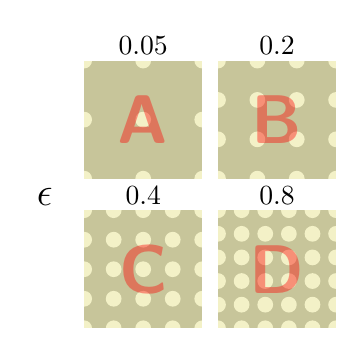
\begin{tikzpicture}
    \tikzset{%
        pics/epsilon/.style args={#1/#2/#3}{code={%
                        \tikzmath{%
                            \dpore=0.1;
                            \deltafig=1.5;
                            \numpore=#1;
                            \deltawall=(\deltafig-\numpore*\dpore)/\numpore;
                        };

                        \begin{scope}
                            \clip (0, 0) rectangle ++(\deltafig, \deltafig);
                            % GDL
                            \fill [GDLcolor] (0, 0) rectangle ++(\deltafig, \deltafig);
                            % pore
                            \foreach \i in {0, ..., \numpore} {%
                                    \foreach \j in {0, ..., \numpore} {%
                                            \fill [white] ({\i*(\dpore+\deltawall)}, {\j*(\dpore+\deltawall)}) circle (\dpore);
                                        }
                                };
                            % EL
                            \fill [ELcolor, opacity=0.5] (0, 0) rectangle ++(\deltafig, \deltafig);
                        \end{scope}

                        \node at (\deltafig/2, \deltafig-0.05) [above] {\ensuremath{#2}};
                        \node at (\deltafig/2, \deltafig/2) [opacity=0.4] {\sffamily\bfseries\color{red}\fontsize{30pt}{30pt}\selectfont #3};
                    }
            }
    }

    \pic at (0, 0) {epsilon=2/0.05/A};
    \pic at (1.7, 0) {epsilon=3/0.2/B};
    \pic at (0, -1.9) {epsilon=4/0.4/C};
    \pic at (1.7, -1.9) {epsilon=5/0.8/D};
    \node at (-0.5, -0.23) {\fontsize{14pt}{0pt}\selectfont\ensuremath{\epsilon}};
\end{tikzpicture}
\end{document}